\begin{titlepage}
  \newpage
  
  \AddToShipoutPicture*{\BackgroundIm}

  \let\footnotesize\small
  \let\footnoterule\relax
  \let \footnote \thanks

  \baselineskip = 1.4\baselineskip

  \begin{center}
  \setcounter{page}{1}
  
  \textbf{\textcolor{um-red}{\large{THÈSE POUR OBTENIR LE GRADE DE DOCTEUR} \\
  \large{DE L'UNIVERSITÉ DE MONTPELLIER} \\ }}
  
  \vspace*{\baselineskip} 
  \normalsize{\textbf{En \specialty}} \\
  \vspace*{\medskipamount} 
  \normalsize{\textbf{Ecole doctorale GAIA}} \\
  \vspace*{\medskipamount}
  \normalsize{\textbf{\department}} \\
  \vspace*{2cm}
  
  \textcolor{um-gray}{\Large{\textbf{\title}} \\ }
  \vspace*{1cm}
  
  \normalsize{\textbf{Présentée par \author}} \\
  \normalsize{\textbf{Le \date}} \\
  \vspace*{\baselineskip}
  
  \normalsize{\textbf{Sous la direction d'\supervisor}} \\
  \vspace*{\fill}
  
  \normalsize{Devant le jury composé de} \\
  \begin{table}[h]
    \centering
    \makebox[0.9\columnwidth]{%
      \begin{tabular}{lllr}
        Prénom NOM             & Titre              & Affiliation                    & \emph{Rôle jury} \\
        Prénom NOM             & Titre              & Affiliation                    & \emph{Rôle jury} \\
        Prénom NOM             & Titre              & Affiliation                    & \emph{Rôle jury} \\
        Prénom NOM             & Titre              & Affiliation                    & \emph{Rôle jury} \\
        Prénom NOM             & Titre              & Affiliation                    & \emph{Rôle jury} \\
        Prénom NOM             & Titre              & Affiliation                    & \emph{Rôle jury} \\
        Prénom NOM             & Titre              & Affiliation                    & \emph{Rôle jury} \\
      \end{tabular}
    }
  \end{table}
  \end{center}
  
  \vspace*{\fill}
  
  \begin{center}
  
\includegraphics[width=0.4\columnwidth]{img/logo-um.png}
  \end{center}
  
\end{titlepage}

\cleardoublepage
  \null\vfill
  \begin{figure}[h!]
  \centering
    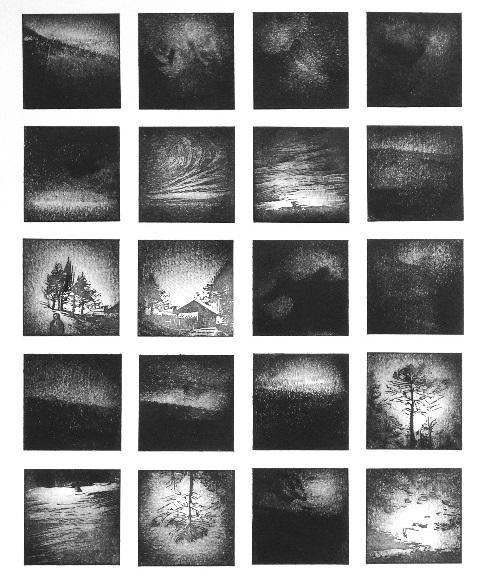
\includegraphics{img/cecile_rescan/cecile_rescan_page.jpg}
    \caption*{Linogravure réalisée par Cécile Rescan}
  \end{figure}
  \vfill\null